\section{Implementation of a counter \\ application}
\label{sec:implementation}
As already mentioned at~\ref{subsec:motivation} this chapter describes the underlying work for this paper and will guide through the entire development process of Electron and Tauri applications.
To obtain comparable results, the methodology of comparison will be explained shortly.
For this paper a basic counter application has been implemented in both Electron and Tauri using just bare \ac{HTML},\ac{CSS} and JavaScript, although both frameworks are supporting most common frontend frameworks like Angular, React or Vue.js.
This decision was made because the paper focuses on presenting the differences and similarities of each framework to the reader and thus using complete frameworks will both blow up the entire application and not concentrate on the essentials.
The counter application consists of a simple Counter which is displayed and two buttons providing the possibility to increment or decrement the counter.
Both buttons will have an event listener, that sends \ac{IPC} messages to the backend and as response get the new calculated counter value which then will be displayed to show the entire communication chain of each framework.
Therefore, each application will contain the same \ac{HTML} content that is displayed and only the \ac{API} calls of the frameworks will differ, depending on their architecture.
To avoid unnecessary distortion of measurements only the fundamentals of each framework are included without any additional helper libraries for better styling or further functionalities.

%This section will include a short explanation of the counter app as an example application.
%It will show the features and define the requirements for an objective comparison.

\subsection{Methodology}
\label{subsec:method}
For benchmarking the applications in case of build time GitHub Actions are used.
Thus, each project has its own GitHub repository with a workflow.yaml defining the Actions' workflow.
Each Action will run on the three major operating systems macOS, Windows and Linux, set the prerequisites for the framework respectively and use the recommended build tool, \texttt{electron-forge} for Electron and the \texttt{tauri build} command for Tauri.
This will result in three jobs for each project, whereas the build time for each framework on each os will be measured, since usual prerequisites are installed once and thus not measured.
Time of execution is measured using hyperfine\footnote{\url{https://github.com/sharkdp/hyperfine}} which is a command line benchmark tool.
Therefore, the executable of each framework will be started by command line, with hyperfine switched in front.
To see the difference between a cached and uncached execution, the first run does not have any warmup actions and so prevent the operating system from loading the application into the filesystem cache.
This results in following command: \shellcmd{hyperfine --runs 10 --warmup 2 'start <executable>}
To gather meaningful data, hyperfine will run 10 instances of the executable to obtain a min-max range as well as a mean execution time with its standard deviation.

For memory consumption the python library memory-profiler\footnote{\url{https://pypi.org/project/memory-profiler/}} will measure the memory consumption of each executable over a timespan of 60 seconds,
enough to allow interactions with the application as well as getting from startup to idle state.
Since the applications rely on multiprocess models and may also spawn child processes, these are recorded too, to gather trustful memory consumption measurements.
To archive this measurement following memory profiler command is used: \shellcmd{mprof run --include-children --multiprocess --timeout 60 <executable>}
It is important to notice that Tauri comes with a single executable file, whereas Electron ships with an installer which has to be executed first in order to get the actual executable application running.
All Electron measurements will use this installed executable as foundation.

Except build time for different operating systems which will use GitHub Actions, the measurements of execution time, memory consumption or binary size
are run on Windows 11.
The implemented application is based on Electron Version 19 the newest stable release at time of writing this paper respectively Tauri version 1.0.2.

%This subection section will take the findings of~\ref{sec:electron} into action and analyze the development and building process as well as the performance of the executable application.

\subsection{Development}
\label{subsec:impl:dev}
The development process is following the best practices section of each framework~\cite{ElectronDoc,tauri} to avoid deprecated or inefficient calls.
Implementation is done with usage of Visual Studio Code, a common, lightweight \ac{IDE} commonly used for web development and also recommended by both Electron and Tauri.

\subsubsection{Prerequisites}

Since Electron mainly relies on Node.js, this as well as the actual Electron framework are the only dependencies that are needed to start developing.
It should be noticed, that Electron is installed as dev dependency since packaged applications are shipped with an Electron binary and therefore are not needed to be defined as production dependency~\cite{electron-in-action}.
Although they are not used, since the application is based on just \ac{HTML} \ac{CSS} and JavaScript, Electron provides several tools for generating a project with fundamental boilerplate code for most common web frameworks like Angular or React.\\
Tauri in contrast needs several more prerequisites to start developing which includes WebView2, the actual web engine for Windows that is used by Tauri as well as Rust, what on the other hand pre-conditions Microsoft Visual Studio C++ Build tools.
Since Tauri consists of two subprojects, the Rust Core and the Frontend it provides a tool for scaffolding boilerplate projects using the most common web-frameworks as well as just plain \ac{HTML} \ac{CSS} and JavaScript (called Vanilla.js by Tauri),
whereas Node.js as prerequisite is implied too.
To initiate the Rust project, once the entire project is scaffolded, the CLI module of Tauri is required.
This tool will generate a minimal Rust project set-up to use Tauri with the selected web-framework and specify the location of all the belonging web assets.

Once each project is initialized a basic \ac{HTML} file combined with basic \ac{CSS} styling is created to specify the actual appearance of the application.
The main JavaScript file of the frontend is specified inside the \texttt{package.json} of each framework.
As mentioned before, two buttons will be added to increment or decrement the counter for invoking a basic \ac{IPC} chain.
Therefore, each button has an event listener which will listen to click events and call the appropriate \ac{IPC} handlers.

\subsubsection{Implementation - Electron}
\label{subsubsec:impl:electron}
Following best practices the Electron framework is divided into three JavaScript files, whereas the main process \\(\texttt{electron.js}) represents core process as described in chapter~\ref{subsec:electron:architecture}.
This file contains the actual browser creation which will spawn a new renderer process  with the corresponding preload script as well as specifications of the content that should be loaded inside the window.
But also required handlers of the \texttt{ipcMain} module including the logic are implemented here.
The second JavaScript is the preload script that contains the \texttt{contextBridge}  and \texttt{ipcRenderer} modules of Electron and exposes the \ac{API} to the renderer process.
This preload script is linked to the main process at the definition of the browser window, that is created by the \texttt{electron.js} file.
The third JavaScript file is the renderer script, that is responsible for adding basic interaction processing that can occur.

\begin{lstlisting}[language=JavaScript,label={lst:rendererjs}, caption={Excerpt of render.js}]
inc_btn.addEventListener('click', async () => {
    counter.innerText =
        await window.electronApi.increment(document.getElementById('counter').innerText)
})
\end{lstlisting}
\begin{lstlisting}[language=JavaScript,label={lst:preloadjs}, caption={Excerpt of preload.js}]
contextBridge.exposeInMainWorld('electronApi', {
    increment: (param) => ipcRenderer.invoke('incrementChannel', param)
})
\end{lstlisting}
\begin{lstlisting}[language=JavaScript,label={lst:electronjs}, caption={Excerpt of electron.js}]
ipcMain.handle('incrementChannel', async(param) => {
    return parseInt(param) + 1;
})
\end{lstlisting}

Once a button is pressed a click event will be emitted and the code shown at listing~\ref{lst:rendererjs} will be executed.
Inside the event listener the related function of the \ac{API}, that is exposed by the preload script and shown at listing~\ref{lst:preloadjs}, will be called.
This will invoke the \texttt{ipcRenderer} module which takes the params of the \texttt{increment} function and send a message using the defined channel, at this case \texttt{incrementChannel} and wait for the response of the handler of the
\texttt{ipcMain} module at listing~\ref{lst:electronjs}.
Since the handler is inside the \texttt{electron.js} which is the main process of the application, this is the place where node modules can be imported and thus the only way for renderer process to use them.
The handler will return the new calculated passed parameter back to the \texttt{ipcRenderer} which then will be set as new counter value as it can be seen at listing~\ref{lst:rendererjs}.
Addressing the difficulty of implementing an application with Electron is has to be said that the entire app can be written with JavaScript,\ac{HTML} and \ac{CSS} which may have a great impact
on small teams of web-developers that are already familiar with those web technologies.
The framework itself is well documented including examples that cover of most use cases and constantly updated to follow the recommendations of the newest releases by the maintainers.
Since Electron uses Node.js as runtime it benefits from its huge community providing libraries for almost any scenario.
Nevertheless, since Electron has released up to 19 stable release versions, there has changed a lot over the years, causing developers to update their applications constantly, which in worst case could result
in reimplementing the entire process communication to migrate their codebase.
\subsubsection{Implementation - Tauri}
Once the two subprojects of the Tauri application are initialized the same frontend as described in chapter~\ref{subsubsec:impl:electron} will be added to the specified web assets folder,
containg the \ac{HTML} file, a \ac{CSS} stylesheet as well as the JavaScript file for processing interaction events, at this example the EventListener of both buttons.

\begin{lstlisting}[language=JavaScript,label={lst:indexjsTauri}, caption={Excerpt of index.js}]
incBtn.addEventListener('click', function() {
    invoke('inc', {cnt: parseInt(counter.innerText)}).then((response) => counter.innerText=response)
})
\end{lstlisting}

\begin{lstlisting}[language=Rust,label={lst:mainrsTauri}, caption={Excerpt of main.rs}]
#[tauri::command]
fn inc(mut cnt: i32) -> String {
  cnt+=1;
   return cnt.to_string();
}

fn main() {
  tauri::Builder::default()
    .invoke_handler(tauri::generate_handler![inc])
    .run(tauri::generate_context!())
    .expect("error while running tauri application");
}
\end{lstlisting}
The core process as described in section~\ref{subsec:tauri:architecture} is created by the \texttt{main.rs} file of the Rust project inside the main function of listing~\ref{lst:mainrsTauri}.
Inside the main method the default function of Tauris Builder structure is executed which will set WRY as runtime for the application.
The \texttt{invoke\_handler} method will set up the passed handlers of the application that will be responsible for \ac{IPC}.
Inside the \texttt{run} method, that will execute the passed context, the actual context is generated by the \texttt{generate\_context} method, that will read the config file, which is the \texttt{tauri.conf.json} by default and create the context of the application.
To indicate handlers that will be executed once the frontend makes an \ac{IPC} request to the core, Tauri uses the \texttt{\#[tauri::command]} makro for commands and \texttt{\#[tauri::event]} for events respectively.
As it can be seen at listing~\ref{lst:indexjsTauri} once a button is pressed, the implemented event handler will be called. 
This will call the \texttt{invoke} method of the Tauri \ac{API} which can either be imported as npm package or set to global inside the config file.
The method takes two parameters whereas the first defines the name the command that should be executed, similar to the channels of Electron and the second parameter is containing all data that should
be passed to the command method and is returning a promise which then can be processed.
Since Tauri is using a protocol similar to \ac{JSON-RPC} the passed data has to be serializable.
After the \ac{IPC} request has reached the core, the corresponding method will be executed which can be seen in listing~\ref{lst:mainrsTauri}.
The command takes integer as parameter, increments it and then returns a string, that will be wrapped into a promise.
After the invoke method returned the promise which contains the processed data of type string it will update the counter.
Referring the complexity and difficulty the reader should keep in mind that implementing a Tauri application nowadays requires knowledge with Rust, since the backend and therefore the process communication can only be implemented in Rust.
Although the Tauri developers announced plans to provide the support of different languages for the backend at the time, this paper is written, it only supports Rust as backend language~\cite{tauri}.
The documentation of Tauri tries to follow the same schema as Electron but is often indistinct and ambiguous or does not provide any detailed information of subjects.
Especially the choice of using Rust as backend the libraries provided by Rusts package manager cargo are limited in contrast to Node.js and may result in writing own libraries to add required functionalities more often.
%As mentioned at~\ref{subsec:electron:architecture} the main process of Electron is running inside the Node.js environment, meaning that this is the only place where Node-Modules can be \textbf{required} and used.
%At this subsubsection the general development process of an Electron application is discussed but also the actual development using the screencast
%application as an example.
%Are there any templates provided, which dependencies and tools are needed for implemention, debbuging and testing.
%Are they already provided by the installer?
%Also have a short look at the documentation e.g.are there any guides, community feedback.

\subsection{Performance}
\label{subsec:impl:performance}
Once the applications are implemented the build process of each framework is invoked to create an executable which is the foundation of performance measurements.
The build time for each application is measured using GitHub actions, whereas it has to be mentioned, that this will be done on completely bare metal runners, that did not cache anything to obtain more comparable measurements
since each framework may cache at different scales.
After the executables are created the performance of both are measured using the techniques described in chapter~\ref{subsec:method}.

\subsubsection{Build Time}
\label{subsubsec:perf:buildtime}
Table~\ref{table:buildingtime} summarizes the results of the GitHub Actions for each operating system and the binary size.
It is clearly visible that building a Tauri app requires much more time than Electron applications spread over the operating systems.
This can be explained with the complex process of Rust compilation like incremental compilation techniques or time-consuming code analysis~\cite{rustCompileTime} combined with the absence
of caching since the GitHub Actions were executed on bare-metal systems.
This is owed due to the fact of providing comparable results and may not occur at every-day development where applications are build constantly to test features and therefore cached to reduce compile time.
\\
\begin{tabular} {| c | c | c | c | c |}
    \hline
    \multicolumn{4}{|c|}{Building time in seconds} & \\ \hline
    Framework & \multicolumn{3}{|c|}{Operating System} & Size [KB]  \\ \hline
    & Windows & Ubuntu & MacOS &  \\ \hline
    Tauri & 863 & 616 & 389 & $6\,924$  \\ \hline
    Electron & 115 & 121 & 44 & $145\,361$ \\ \hline
\end{tabular}
\label{table:buildingtime}
\\ \\

The binary size of the compiled executable amounts to $6\,924$ kB for the Tauri application respectively $145\,361$ kB for Electron which is a direct result of the architecture of both framework described in chapters~\ref{subsec:electron:frontend} and~\ref{subsec:tauri:frontend}.
Electron ships the executable with an entire web browser whereas Tauri makes use of the system specific web engine and therefore is able to reduce its size by a factor of approximately 21.
This may be an advantage or disadvantage depending on the developers or customers point of view, since the different web engines of each system result in slightly different appearances of the application.

\subsubsection{Memory Consumption}
\label{subsubsec:perf:memory}
\figref{fig:electron:memory} and \figref{fig:tauri:memory} show the entire memory usage of the implemented applications including their child processes.
Although the Electron application consumes more memory at startup, causing a peak of approximately 400 MiB at \figref{fig:electron:memory} it decreases its memory consumption up to approximately 290 MiB,
whereas the Tauri Application is constantly at a consumption of roughly 320 to 330 MiB\@.
Both figures also point out that Tauri has more processes involved into the application than Electron.
Those graphics stay in contrast to the actual benchmarks provided by Tauri\footnote{\url{https://tauri.app/about/benchmarks/}} and thus only the benchmarks for Electron are made public it is not possible to explain the discrepancies between both frameworks objectively.
\begin{figure}[ht]
    \centering
    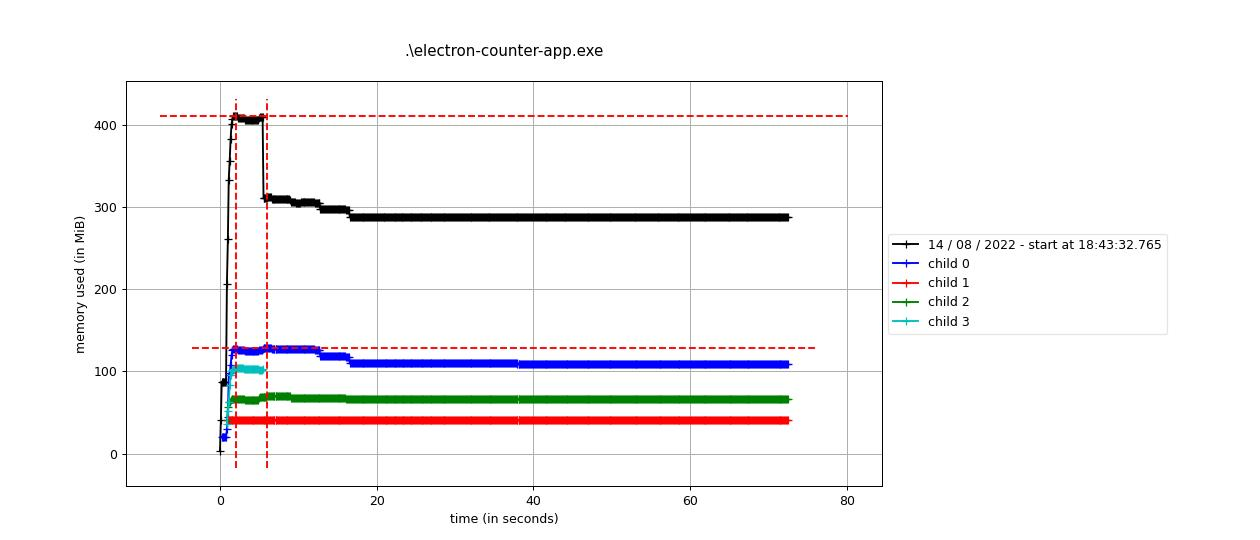
\includegraphics[width=0.5\textwidth]{images/ElectronMemCons}
    \caption[]{Memory consumption of Electron executable obtained from memory profiler}
    \label{fig:electron:memory}
\end{figure}
\begin{figure}[ht]
    \centering
    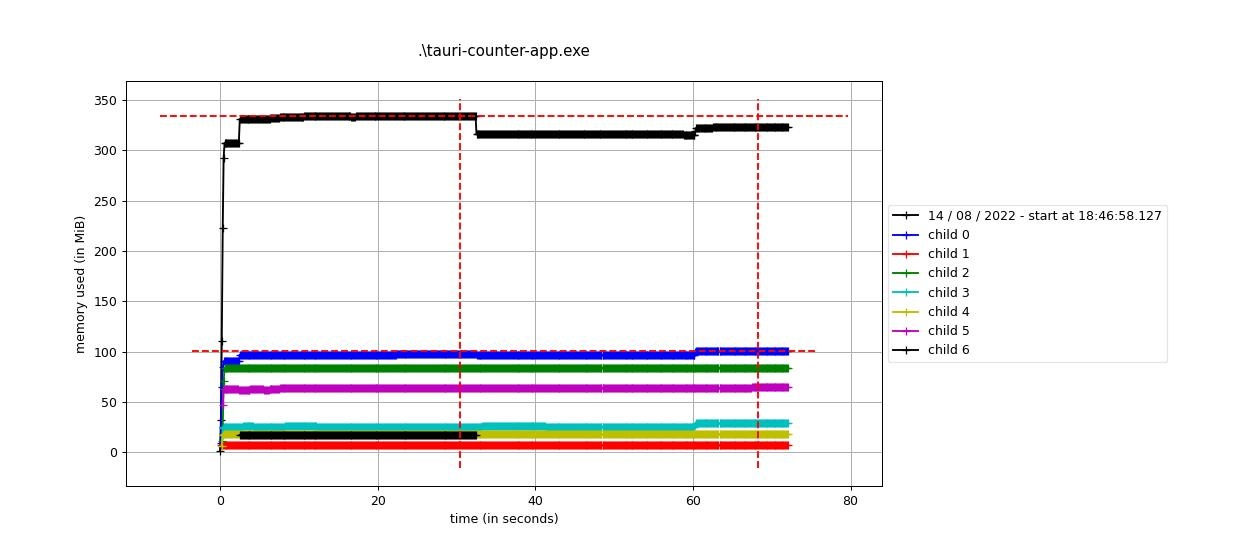
\includegraphics[width=0.5\textwidth]{images/TauriMemCons}
    \caption[]{Memory consumption of Tauri executable obtained from memory profiler}
    \label{fig:tauri:memory}
\end{figure}
\\
\subsubsection{Execution Time}
\label{subsubsec:perf:execution}

The measurements of \texttt{hyperfine} are shown below, whereas the mean values include their standard deviation based on ten measurements and caching describes the warmup option that is added to the second run of hyperfine.
The high standard deviation of both table~\ref{table:exec:electron} and table~\ref{table:exec:tauri} at the \textbf{Without caching} row can be explained with the max values of the same row.
The max value is more than 2 standard deviations away from the mean value meaning it is not a probable execution time, but it also shows the effect of filesystems caching.
To obtain more reliable and undistorted measurements the warmup option of hyperfine is included at the values of the \textbf{With caching} row showing the results of execution time after the application is cached.
Both tables point out, that the execution time of the Tauri application is faster than the Electron application at all measured values even if the mean values of Electron and Tauri only slightly differ.
This is reasoned by Tauris' usage of Rust as backend which has a performance similar to C++~\cite{rustPerformance} and thus is more performant than JavaScript~\cite{C++Javascript}.

\begin{tabular} {| c | c | c | c |}
    \hline
    \multicolumn{4}{|c|}{Execution time of Electron [ms]} \\ \hline
     \multicolumn{4}{|c|}{}\\ \hline
     & Mean   & Min & Max     \\ \hline
    Without caching & 17.3 $\pm$ 23.3 & 6.5 & 82.9  \\ \hline
    With caching & 18.0 $\pm$ 14.8 & 7.5 & 49.6 \\ \hline
\end{tabular}
\label{table:exec:electron}
\\ \\

\begin{tabular} {| c | c | c | c |}
    \hline
    \multicolumn{4}{|c|}{Execution time of Tauri [ms]} \\ \hline
    \multicolumn{4}{|c|}{}\\ \hline
    & Mean & Min & Max     \\ \hline
    Without caching & 17.1 $\pm$ 10.5 & 5.8 & 35.4  \\ \hline
    With caching & 15.1 $\pm$ 7.9 & 5.2 & 29.0 \\ \hline
\end{tabular}
\label{table:exec:tauri}
\\ \\
%At this subsubsection the actual performance of the example application is analyzed.
%Memory consumption, known security issues, bugs, freezes etc.
%This subsection section will take the findings of~\ref{sec:tauri} into action and analyze
%the development and building process as well as the performance of the executable application.
